
\chapter{引言}
\label{chap:intro1}

\section{研究背景}

\subsection{为什么要不断提升计算能力?}

在过去的半个多世纪中,计算能力的不断提升已经成为许多行业飞速发展(如科学计算、互联网、娱乐等)的核心力量。例如:人类基因解码、更准确的医疗成像、更快速精确的网络搜索、更真实的电脑游戏等,都离不开计算能力的提高。

随着计算能力的提升,应用软件可以帮助我们完成更多、更复杂的工作,推动科学研究的进步。随着更复杂的科学问题的提出,也会对计算能力提出更高的要求,更加具有挑战的问题也越来越多,如下有一些例子:

\begin{itemize}
	\item 气候模拟:为了更好的理解气候变化,需要更加精确的计算模型,这种模型需要对大气、海洋、陆地以及极地冰川之间的关系做详细的研究,会涉及到超大规模数据的处理。
	\item 蛋白质折叠:人们相信错误折叠的蛋白质与亨廷顿病、帕金森病、老年痴呆症等疾病有千丝万缕的联系,但是现有的计算性能严重限制了研究复杂分子(如蛋白质)结构的能力。
	\item 能源研究:不断提高的计算能力可以为某些技术(如风力涡轮机、太阳能电池和蓄电池)构建更加详细的模型。这些模型能够为建立更加高效清洁的模型提供信息。
	\item 数据分析:各行各业每天都会产生大量的数据。据统计,全球范围存储的数据每两年翻一番,而且增速仍然呈上升趋势,但是这些数据中的大部分在未经分析之前并不能发挥价值。
\end{itemize}

要解决上述问题,需要进一步提高计算机的计算能力\citep{pacheco2011introduction}。

\subsection{单核处理器的性能提升达到瓶颈}

处理器性能的提升是提高计算机的计算能力的方式之一,在很长一段时间里,只依靠处理器性能的提升就可以满足各种软件对计算能力越来越高的需求。但是随着处理器性能的增幅降低,提高计算能力已经不能仍然完全依靠处理器性能的提升了。

\begin{figure}[!htbp]
    \centering
    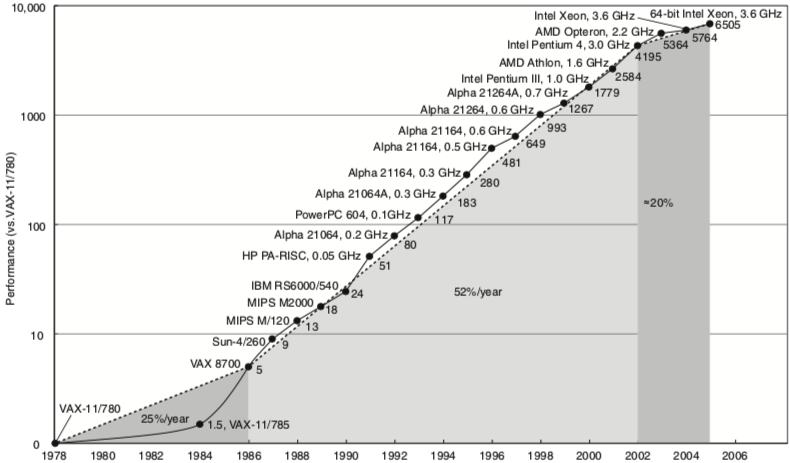
\includegraphics[width=0.40\textwidth]{hist_proc}
    \bicaption{自80年代中期以来处理器性能的增长。}{Growth in processor performance since the mid-1980s.}
    \label{fig:hist_proc}
\end{figure}

如图1.1\citep{edwards2011arch}所示,从1986年到2002年,单核处理器的性能以平均每年超过50\%的速度不断提升等问题的出现,用户和软件开发人员只要等待下一代处理器发布,就可以获得应用程序性能的提升。

但是随着CPU制造工艺逼近物理极限、主频提升导致功耗急剧增加,从2003年开始单核处理器的性能提升速度就大大降低了,降为20\%左右。这个差异是巨大的,如果性能提升速度是50\%,在10年的时间内性能提升可以达到60倍;如果提升速度只有20\%,10年内只能提升6倍\citep{pacheco2011introduction}。近年来,随着大数据时代的到来,数据量每年都在成倍地增长,每年20\%的计算能力的提升显然是不够的。

在这种情况下,CPU生产商改变策略,不再将主要精力放在构建更快、更复杂的单核处理器,而是转向多核技术,通过在同一芯片上集成多个处理器的方法来提升CPU的性能。同时,计算机硬件和体系结构也从早期的大型主机、向量机转向分布式的低成本的x86 PC的集群架构,集群中的节点也逐渐由单处理器更新为多核处理器。分布式的计算机集群为算法的加速和应用的可扩展性提供了另一种方式。

\subsection{并行计算的发展}

近年来,CPU频率的上升已经接近尾声,依靠硬件性能提升来获取软件性能提升的“免费午餐”时代已经结束。随着单CPU的多核化,并行计算已经不是超算领域所独享的技术,分布式并行编程逐渐成为应用软件、数值计算库乃至工具开发的基本编程方式,开发性能优越的软件的门槛逐渐提高,甚至具有相当的挑战性。为了进一步提升软件的性能,只能通过充分发挥多核处理器和分布式集群的性能来实现,软件开发人员不得不考虑并行编程。

然而多核处理器和分布式集群所提供的性能提升不是免费的,到目前为止,自动并行化领域始终没有重大的进展。尽管某些编译器可以并行化一些非常简单的代码,但是效果并不理想,对于稍微复杂些的程序基本上都无能为力。因此,发挥多核处理器性能的责任基本上完全落在了软件开发人员的肩上,而目前没有很好的并行编程工具可用\citep{liuwenzhi2015paraalgo}。

当前常见的并行环境大体可以分为共享内存并行和分布式内存并行:
\begin{itemize}
	\item 共享内存并行:所有控制流都能够访问一个共同的内存地址空间,通过这个内存来交换数据。目前基于多核处理器的并行环境基本上都是共享内存并行环境,比如pthread、OpenMP等。共享内存并行的通信代价较小,但是对共享数据的访问需要开发人员显式处理,保证程序的正确性。
	\item 分布式内存并行:通过网络互连的多机系统、存储器分布在不同节点上,每个节点运行各自的操作系统,拥有独立的物理地址空间。由于通过网络互连,控制流之间的通信只能通过网络数据传输实现。目前常用的分布式内存并行编程环境是MPI(消息传输接口),MPI已经是事实上的标准。由于每个控制流拥有独立的内存地址空间,所以不存在内存访问冲突,多控制流之间的协调通信比较复杂。
\end{itemize}

并行编程方式与串行编程方式相比要复杂得多,要求开发人员不仅要考虑软件本身的架构和逻辑,还要通过显式的并行编程来实现多核环境下任务和数据的划分、对临界资源并发访问的控制、多个控制流之间依赖关系的维护等复杂的问题。所以并行编程对软件开发人员的要求非常高,需要丰富的系统结构的知识沉淀和并行优化技术的经验积累,还需要很大的工作量(因为开发工具不智能)。这给许多软件开发人员带来巨大的挑战,增加了开发的难度。尤其是那些非计算机专业的、从事其他科学研究工作的开发人员,他们往往对计算机科学了解不深刻,习惯于用串行编程方式来实现算法,并行优化对他们来说难度过大,学习成本过高,妨碍他们将主要精力放在研究算法本身。

所以,并行优化的研究具有重要的意义,需要继续投入科研力量去推进并行优化技术的发展,从而进一步提高计算资源的使用效率,提供简单易用的API,为软件开发人员提供优秀的并行编程工具。

\section{研究动机}

随着多核处理器和分布式集群的普及,并行编程在高性能计算领域和互联网软件开发中的作用越来越大。但是到目前为止,并行编程的开发环境还较为落后,传统的并行编程技术以及科学计算库难以充分利用如今计算机体系架构下的多核机和分布式集群的性能,造成计算资源的浪费,难以达到优秀的性能提升效果。

MPI作为分布式内存下并行编程的标准已经有二十多年的历史,它有很多明显的缺点:需要通过显示的消息传递实现控制流的并行执行,使用难度较高,而且不能充分利用单机中的多核,往往需要结合多线程编程技术如pthread和OpenMP等,这样的话又要考虑共享内存环境下线程安全等问题\citep{hwu2008concurrency}……

使用MPI+pthread/OpenMP在多核节点构成的分布式集群进行并行编程,不仅编程复杂,而且调试困难,将给开发人员带来极大的挑战。如何代替开发人员在多核和分布式环境下进行并行优化,提高计算资源的利用率和程序的性能,是亟待解决的问题。

从并行计算模型上来看,传统的BSP(Bulk Synchronous Parallel)计算模型\citep{cheatham1996bulk}的设计特点是存在整体同步。一个BSP程序由一系列超步组成,超步内的任务可以并行执行,超步之间则是顺序执行的(如图1.2所示)。

\begin{figure}[!htbp]
    \centering
    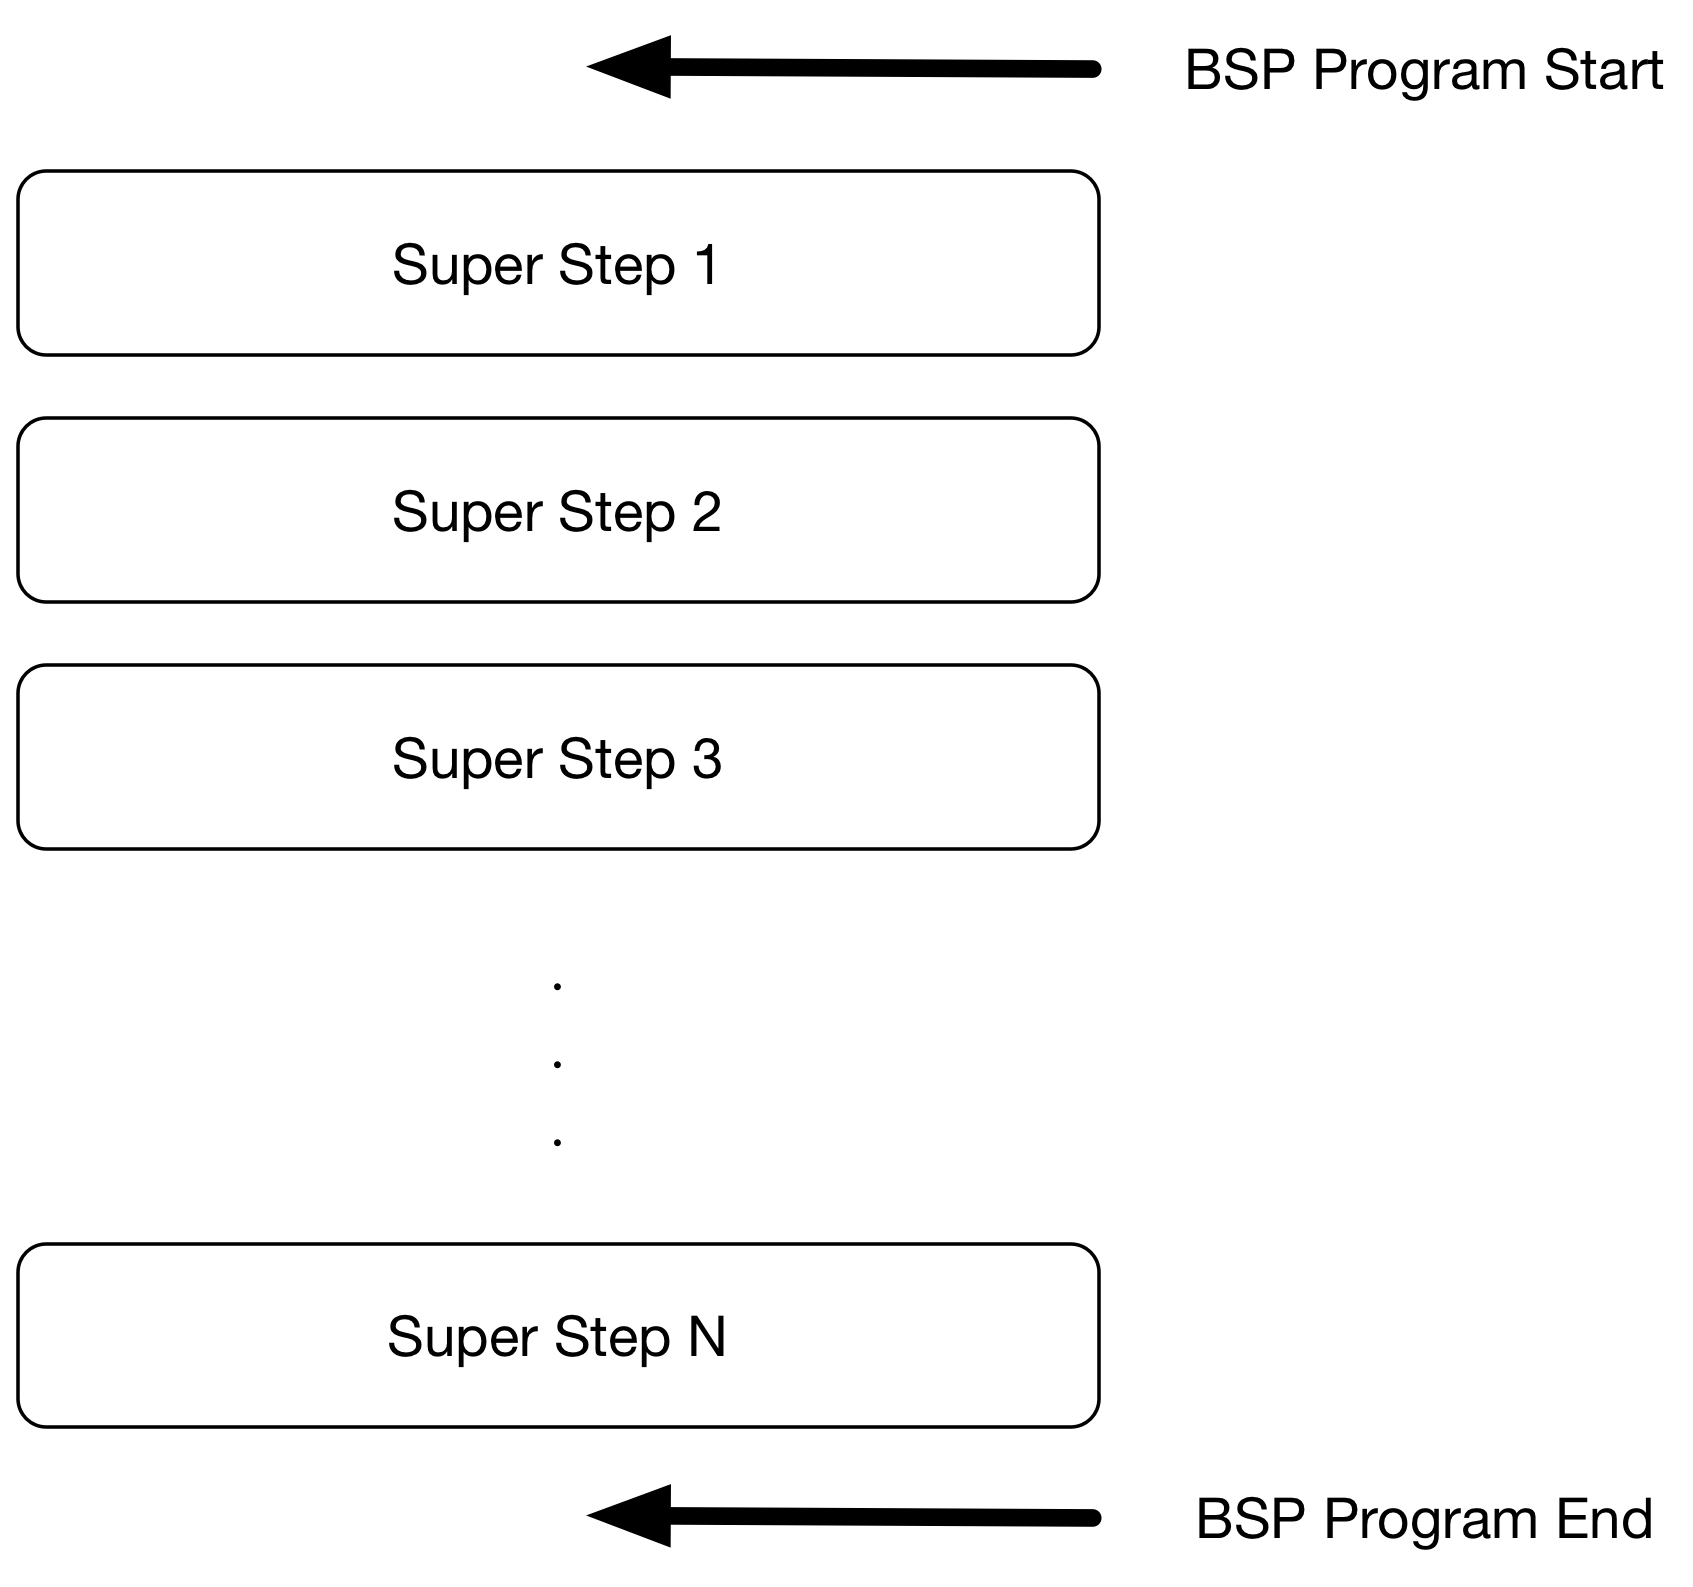
\includegraphics[width=0.40\textwidth]{bsp_super_step}
    \bicaption{BSP计算模型中的超步。}{Super steps in BSP computing model.}
    \label{fig:bsp_super_step}
\end{figure}

在一个超步中,所有的控制流并行执行局部计算,然后进行全局通信,最后在同一个路障(barrier)处同步( 如图1.3所示)。

\begin{figure}[!htbp]
    \centering
    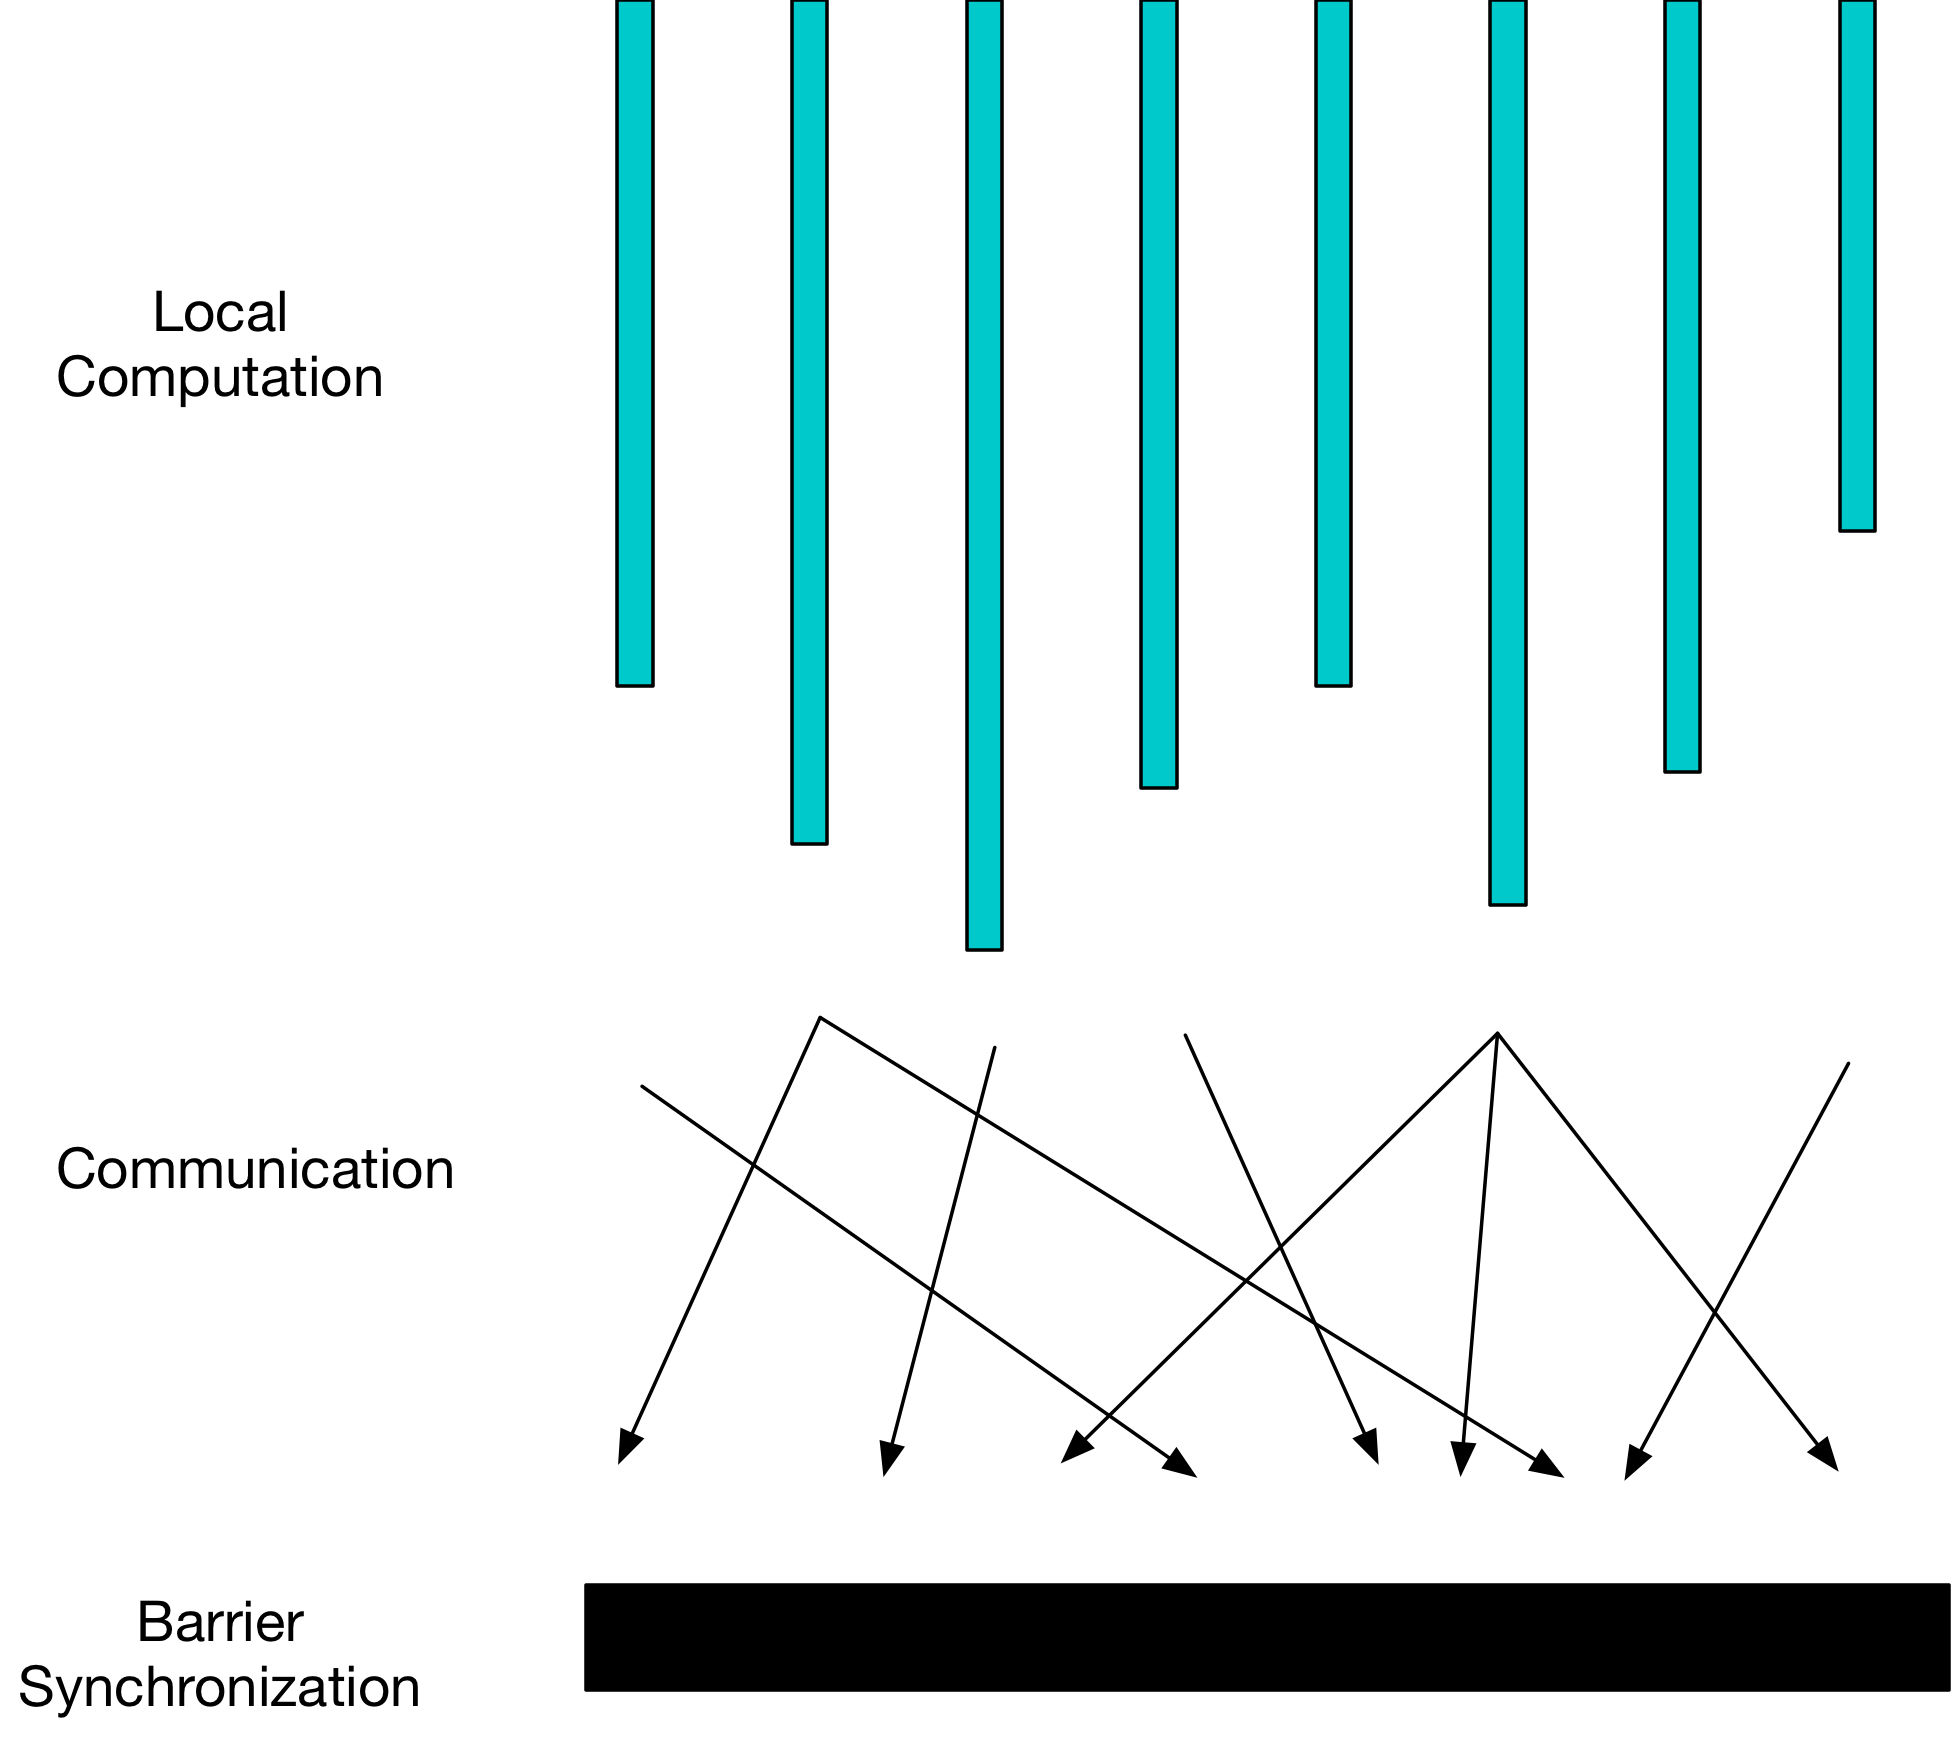
\includegraphics[width=0.40\textwidth]{bsp_super_3steps}
    \bicaption{BSP计算模型中超步的3个阶段。}{Three phases in a super step in BSP computing model.}
    \label{fig:bsp_super_3steps}
\end{figure}

BSP计算模型简化了并行算法的设计和分析,但是牺牲了运行时间,因为整体同步会导致同一超步内的所有控制流必须等待最慢的执行单元结束后才能继续推进。当分布式节点或节点不同核心的计算时间差异较大时,会造成更多的运行时间的浪费。

相比之下,数据流模型则克服了这个缺点。数据流模型是一种天然的并行模型,不需要集中控制,对于任何一个任务,只要它的输入就绪,当运行时有可用资源就可以开始运行,这样就大大提高了计算资源的利用效率,可以实现超大规模的并行。

从并行编程模型上来看,OpenMP是当今科学计算领域最重要的共享内并行编程模型,共享内存具有统一的地址空间,可以直接访问数据,易于编程,但是要考虑线程安全等问题;MPI是当今面向分布式内存计算的最重要的并行编程模型,分布式内存的地址空间是分散的,数据的共享要用过消息传递来实现,编程比较复杂,但是可以获得更好的可扩展性。而分区全局地址空间(PGAS,Partitioned Global Address Space)编程模型则结合了共享内存和分布式内存的优点,同时具备了共享内存编程模型的高效率、易编程性和分布式内存编程模型的可扩展性。

我们计划投入科研力量,研发更加高效、易用的并行优化工具,提供在单机多核环境和分布式集群环境下的通用的并行优化解决方案,支持数据流模型和PGAS模型,包含高效的任务调度策略。开发这种并行优化工具的主要目标是:

\begin{itemize}
	\item 提供简单易用的并行编程API,提高并行开发效率,缩短并行编程的开发周期。
	\item 提高计算资源利用率,充分发挥有限的硬件资源的性能。
	\item 同时支持共享内存环境和分布式内存环境,易编程,可扩展性高。
	\item 缩短科学大数据应用并行化的移植周期,提升科学研究的效率。
\end{itemize}

\section{本文主要贡献}

本文分析了目前并行编程技术的发展和面临的挑战,从并行计算模型和并行编程模型两个方面找到了构建更加高效、易用的并行优化工具的方向:采用数据流计算模型解决传统BSP模型全局同步造成的计算资源浪费的问题,采用PGAS并行编程模型来结合共享内存并行编程模型的易编程性和分布式内存并行编程模型的可扩展性。之后按照这个思路分别实现了共享内存下基于线程池和数据流计算模型的并行优化工具star\_tp和分布式内存下基于PGAS和数据流计算模型的star-d,并对它们进行了性能测试。

本文的贡献主要包括以下三个方面:

\begin{enumerate}
	\item 设计并实现了共享内存下基于线程池和数据流计算模型的并行优化工具——star\_tp。线程池的使用减少了线程创建和销毁造成的系统开销,任务调度基于任务之间之间的依赖关系,没有依赖关系的任务可以异步执行,减少了不必要的等待时间,从而提高了CPU的利用率,进而提高应用程序的性能。
	\item 设计并实现了分布式内存下基于PGAS和数据流计算模型的并行优化工具——stat-d。PGAS是一种并行编程模型,编程时,使用PGAS可以向访问本地数据一样访问分布式数据结构。分布式内存版本的任务调度同样基于数据流计算模型,具有良好的可扩展性。
	\item 验证star\_tp和star-d的优化效果。选择中国科学院遥感与数字地球研究所的InSAR (干涉合成孔径雷达)系列算法做为测试用例,这是一个典型的科学大数据应用。首先对每个算法使用OpenMP进行优化,作为对比的基准,然后对InSAR系列算法进行封装,分别在star\_tp和star-d的运行时环境下进行并行优化,最终都获得了优于OpenMP的优化效果。
\end{enumerate}

\section{本文组织结构}

本文的内容分为六章,各章的内容如下:

第一章阐述了研究的背景和动机,分析了当前并行优化的现状,指出了传统的并行编程模型和工具存在的问题。通过对比和分析,决定采用数据流计算模型和PGAS编程模型进行并行优化工具的开发。同时指出了本论文的研究意义和目标。

第二章介绍了当前主流的并行编程模型,包括传统并行编程模型、PGAS模型和数据流计算模型。分析了传统并行编程模型和工具的优势和存在的问题,介绍了PGAS编程模型的兴起和相关的实现,最后介绍了数据流模型。

第三章介绍了共享内存环境下基于线程池和数据流计算模型的并行优化工具——star\_tp的设计和开发,包括star\_tp的架构、API和运行实例。

第四章介绍了分布式内存环境下基于PGAS编程模型和数据流计算模型的并行优化工具——star-d的设计和开发,包括star-d的架构、API和运行实例。

第五章介绍了使用star\_tp和star-d优化中国科学院遥感与数字地球研究所的InSAR系列算法。包括使用OpenMP对InSAR系列算法进行并行优化,优化结果作为对比基准,然后分别将InSAR的算法接口进行简单的封装,分别作为任务插入star\_tp和star-d的运行时环境中进行并行优化。

第六章总结了本论文的所有工作,指出了所做工作的贡献,同时也指出了工作中存在的不足,提出了后续改进的建议。
